\documentclass[electronics,article,submit,moreauthors]{Definitions/mdpi}

\firstpage{1}
\makeatletter
\setcounter{page}{\@firstpage}
\makeatother
\pubvolume{1}
\issuenum{1}
\articlenumber{0}
\pubyear{2026}
\copyrightyear{2026}
\datereceived{ }
\daterevised{ }
\dateaccepted{ }
\datepublished{ }

\Title{Hazard-Coupled Self-Powering and Corridor-Wide Duty-Brokering for Off-Grid Landslide Early-Warning IoT Sensor Swarms: A Design and Simulation Study for Malaysian Highway Cut-Slopes}

\newcommand{\orcidauthorA}{0000-0002-0049-4747}
\newcommand{\orcidauthorB}{0000-0002-5151-2300}

\Author{Subarmaniam Kannan $^{1,2,}$*\orcidA{} and Sumendra Yogarayan $^{1,2}$\orcidB{}}

\AuthorNames{Subarmaniam Kannan and Sumendra Yogarayan}

\address{%
$^{1}$ \quad Faculty of Information Science and Technology (FIST), Multimedia University, Jalan Ayer Keroh Lama, Bukit Beruang, 75450 Melaka, Malaysia\\
$^{2}$ \quad Centre of Intelligent Cloud Computing (CICC), Multimedia University, Jalan Ayer Keroh Lama, Bukit Beruang, 75450 Melaka, Malaysia}

\corres{Correspondence: subar.kannan@mmu.edu.my}

\abstract{Microgrid-powered Internet of Things (IoT) sensing has been shown to sustain continuous monitoring by switching between renewable and utility-grid power sources, but this model assumes utility backup is always available --- an assumption that fails for landslide-monitoring sensor swarms on remote, off-grid highway cut-slopes. (1) Background: we address the gap between the single-node ``IoT microgrid'' architecture validated for grid-adjacent deployments and the off-grid, no-utility-backup conditions typical of landslide-prone highway corridors in Malaysia. (2) Methods: we propose two extensions --- hazard-coupled self-powering, in which a piezoelectric harvester generates power that increases with ground micro-movement rather than decreasing with the solar supply under the same monsoon conditions that drive instability, and corridor-wide duty-brokering, in which nodes reassign sensing duties to neighbors with surplus power --- and evaluate them with a controlled, 50-seed Monte Carlo simulation driven by real solar irradiance data (Kuala Lumpur, full year 2025) and real piezoelectric harvester characterization data (23 laboratory experiments), following a systematic review of 147 sources. (3) Results: duty-brokering reduced sensing downtime during correlated monsoon-front conditions by up to 32.7\% at resource-constrained settings, the finding survived an ablation removing the one unvalidated model component, and a real-data cross-check against an actual highland site and four documented Malaysian landslide incidents produced a mixed but informative result that led us to revise the design, downgrading an originally proposed flow-harvester component after finding it viable for under 1\% of the year. (4) Conclusions: this is reported as a preliminary computational feasibility study, not a field validation, and we specify the hardware-in-the-loop and physical-prototype work still required before deployment.}

\keyword{IoT microgrid; landslide early warning; energy harvesting; piezoelectric; duty cycling; hardware-in-the-loop; wireless sensor network; Malaysia}

\begin{document}

\section{Introduction}

Internet of Things (IoT) sensing has become central to natural-hazard monitoring, but IoT devices require continuous power, and continuous power is the scarcest resource in exactly the remote, off-grid locations where hazard sensing matters most. Lee and Wang~\cite{ref101} address this for grid-adjacent deployments with an ``IoT microgrid'' architecture: a single DC sensor node switches between a renewable primary source and a utility-grid secondary source using a double-voltage-threshold controller, validated on a hardware-in-the-loop (HIL) testbed built around a Speedgoat real-time target machine. Their model rests on four assumptions, the second of which --- that utility-grid power is available as backup --- does not hold for landslide-monitoring sensors on remote highway cut-slopes, a deployment class with no utility access and frequently canopy-shaded or monsoon-obscured solar exposure.

Malaysia provides a concrete setting for this gap. The Public Works Department (Jabatan Kerja Raya, JKR) maintains a hazard-and-risk inventory of 34{,}714 slopes along federal roads nationwide (26{,}722 in Peninsular Malaysia, 4{,}178 in Sabah, 3{,}633 in Sarawak, and 181 in Labuan), of which 1{,}577 are classed high-risk, under the National Slope Master Plan 2025--2030. Historical incidents --- the 1993 Highland Towers collapse, the 2008 Bukit Antarabangsa landslide, and the 2022 Batang Kali campsite landslide (31 deaths) --- demonstrate the consequence of slope failure, while recurring closures on routes such as Simpang Pulai--Cameron Highlands show the continuing operational burden on transportation infrastructure. JKR already operates 49 rainfall telemetry stations (37 in Peninsular Malaysia, 9 in Sabah, 3 in Sarawak) and robotic total stations at selected federal-road sections, yet no system identified in our literature review (Section~\ref{sec:related}) reports a self-powering or inter-node redundancy mechanism for the specific condition where solar power and ground instability change together --- a monsoon-triggered correlation this paper treats as the central design problem.

This correlation is not merely a theoretical concern. A sensor network that relies on solar power to operate continuously faces a structural conflict: the same monsoon rainfall that raises landslide risk through soil saturation also attenuates the solar irradiance the sensor needs to keep operating and reporting. If a node's energy buffer is depleted precisely when a storm front passes, the monitoring system fails at the moment it is needed most. The present study investigates whether this conflict can be resolved at the architecture level, rather than through larger batteries or more frequent maintenance visits, which are themselves difficult to sustain on steep, remote, and frequently inaccessible terrain.

We ask: can hazard-coupled self-powering --- energy harvesting whose output rises with the hazard itself, rather than with ambient weather --- combined with corridor-wide duty-brokering --- task reassignment among spatially distributed nodes over the existing communication link --- sustain network-level sensing continuity for an off-grid landslide early-warning swarm, where the reference architecture's utility-backup assumption cannot be satisfied? We do not answer this with field data; no hardware has been deployed as part of this study. Instead, we establish, through systematic literature review, real-data-grounded simulation, and direct cross-checking against real weather and incident records, that the proposed design is mechanistically sound, identify which of its components are and are not currently well supported by evidence, and specify the validation path required before deployment. Throughout, we apply the same verification standard to our own simulation code that we apply to the literature we cite: two implementation errors discovered and corrected during this work are disclosed rather than silently fixed (Section~\ref{sec:internal-validity}), and one model component found, on testing, not to work as originally proposed is reported as a negative result rather than adjusted until it looked favorable (Section~\ref{sec:flow-result}).

The remainder of this paper is organized as follows. Section~\ref{sec:related} reviews related work across nine technology clusters identified through a systematic search. Section~\ref{sec:design} presents the proposed system design and algorithm. Section~\ref{sec:methods} describes the simulation methodology and the real and modeled data used to drive it. Section~\ref{sec:results} reports results, including a sensitivity sweep, an ablation study, and cross-checks against real weather and incident data. Section~\ref{sec:discussion} discusses implications, internal and external validity, and the revisions this process produced to the original design. Section~\ref{sec:conclusion} concludes.

\section{Related Work}
\label{sec:related}

A systematic, PRISMA-aligned search was conducted across Semantic Scholar, OpenAlex, and PubMed (via a Consensus aggregator interface) using ten thematic queries covering landslide/slope IoT monitoring, rainfall-induced landslide threshold models, piezoelectric and vibration-based self-powered sensing, flow/hydrokinetic energy harvesting, LoRaWAN/LPWAN communication for remote disaster monitoring, IoT microgrid and cyber-physical renewable energy management, energy-aware wireless sensor network (WSN) duty-cycling and clustering, peer-to-peer energy trading in microgrids, and hardware-in-the-loop testbed methodology. From 200 candidate records, duplicates were removed and venue-quality screening was applied: three sources were dropped because their indexing status in Scopus, the Directory of Open Access Journals, or Web of Science could not be confirmed, and one further source, published by a venue with a documented history of large-scale, unrelated peer-review integrity concerns in 2023, was excluded from this manuscript's citation set after we were unable to independently re-verify the specific article within the scope of this study (Section~\ref{sec:verification}). The remaining 146 sources, organized into nine thematic clusters, are cited throughout this review.

\subsection{Landslide and Slope IoT Monitoring Systems}

Thirty of the reviewed systems describe wireless sensor network (WSN) or IoT-based landslide and slope monitoring, spanning deployments in Kerala, India~\cite{ref2,ref12,ref20}; the Darjeeling Himalayas~\cite{ref18}; an informal settlement in Medell\'in, Colombia~\cite{ref14}; and two Malaysian systems, one in Hulu Langat following the 2011 landslide that killed 16 people~\cite{ref21}, and one at Bukit Bauk, Dungun~\cite{ref31}. Reviews of this literature~\cite{ref22,ref23} confirm that landslide WSNs have matured substantially since Ramesh's early Kerala deployments~\cite{ref2,ref12,ref20}, incorporating inertial measurement units~\cite{ref2}, LoRaWAN communication with machine-learning-based risk classification~\cite{ref4,ref5}, geosensor networks for subsurface monitoring~\cite{ref9}, and distributed systems purpose-built for highway embankments~\cite{ref26}. Across this entire cluster, every reviewed system relies on either periodic battery replacement, solar-only backup, or --- where grid-tied --- utility fallback. No reviewed system models a no-grid, node-to-node service-continuity mechanism, which is the specific gap this paper addresses.

\subsection{Rainfall-Induced Landslide Threshold and Prediction Models}

Seventeen sources establish and refine rainfall-intensity--duration and cumulative-rainfall threshold models for predicting landslide occurrence~\cite{ref32,ref33,ref34,ref35,ref36}. These models, several of them region-specific to China~\cite{ref33,ref34,ref37}, Italy~\cite{ref32,ref42,ref43}, and the Himalayas~\cite{ref44,ref46,ref49}, consistently find that landslide risk escalates during sustained or intense rainfall, and that antecedent (cumulative, multi-day) rainfall is frequently a stronger predictor than same-day totals~\cite{ref40,ref45,ref47}. This literature establishes the hazard-signal dynamics --- rainfall intensifying landslide risk with a time lag that can extend over days~\cite{ref48} --- but does not address the power-architecture implication: that the same rainfall simultaneously attenuates the solar irradiance a monitoring node depends on. This structural conflict is not discussed in any source in this cluster.

\subsection{Piezoelectric and Vibration-Based Self-Powered Sensing}

Piezoelectric vibration energy harvesting is a mature, field-validated technology for powering wireless sensor nodes~\cite{ref51,ref55,ref58,ref64}, with reported output power ranging from microwatts~\cite{ref59} to over 100~mW under strong excitation~\cite{ref62}. Critically for this paper's design, two sources already embed piezoelectric elements directly into slope-stabilization geosynthetics --- a geocable--geogrid composite~\cite{ref53} and a ``smart'' geobelt~\cite{ref54} --- using the piezoelectric response to detect strain and microseismic activity within a reinforced slope. Both, however, use the piezoelectric element exclusively for \emph{sensing} (via voltage or impedance signatures), not for harvesting usable \emph{power} to run a wireless node. This distinction --- sensing from ground movement versus powering from it --- is the specific, verified gap this paper's hazard-coupled harvesting design exploits.

\subsection{Flow and Hydrokinetic Energy Harvesting for Remote Sensors}

Fourteen reviewed sources characterize flow-based (hydrokinetic) energy harvesters for wireless sensor applications, including microturbine designs~\cite{ref66,ref71}, triboelectric and electromagnetic hybrid generators~\cite{ref67,ref68}, and broader surveys of the field~\cite{ref69,ref76,ref79}. Reported power output ranges from nanowatts to several hundred milliwatts depending on flow velocity and transduction mechanism~\cite{ref69}, with specific, reproducible power--velocity relationships reported for Savonius-type microturbines operating between 0.5 and 2.0~m/s water velocity~\cite{ref66}. All of this characterization work, without exception, was conducted under clean, controlled flow conditions --- laboratory flow rigs, domestic water pipes, or open water channels --- and none addresses performance under the sediment-laden, intermittent runoff conditions that would be encountered on an actual landslide-prone slope face. This is a field-versus-laboratory validity gap this paper tests directly (Section~\ref{sec:flow-result}).

\subsection{LoRaWAN and Low-Power Wide-Area Network Communication for Remote Disaster Monitoring}

Thirteen sources address Long Range Wide Area Network (LoRaWAN) and related low-power wide-area network (LPWAN) technologies for disaster and environmental monitoring in remote, infrastructure-poor settings~\cite{ref81,ref83,ref84,ref87}, including applications specifically to landslide and rockfall monitoring~\cite{ref86,ref93}. Connectivity reliability under adverse terrain is a recurring, quantified concern: a rural Mozambican deployment reported a packet delivery ratio (PDR) as low as approximately 89\% under terrain- and altitude-constrained conditions~\cite{ref92}, and a Malaysian study of LoRa signal propagation in hilly suburban terrain near Kuala Lumpur found that packet receive ratio could drop by 65\%, with coverage reduced to as little as 1.25~km, across spreading factors SF7 through SF12 at 915~MHz~\cite{ref28}. This Malaysian terrain-degradation finding is, to our knowledge, the closest available match in the literature to the actual highway-corridor communication conditions this paper's duty-brokering protocol must tolerate, and is used accordingly in Section~\ref{sec:design}.

\subsection{IoT Microgrid and Cyber-Physical Renewable Energy Management}

Seventeen sources, including the primary reference architecture~\cite{ref101}, describe IoT-integrated microgrid energy management systems~\cite{ref96,ref97,ref98,ref99,ref100}, reviews of microgrid control and monitoring strategies~\cite{ref102,ref108,ref111}, blockchain- and machine-learning-enhanced approaches~\cite{ref95,ref103,ref105}, and demand-side management frameworks~\cite{ref109,ref112}. One source~\cite{ref104} reports a hybrid photovoltaic/wind/piezoelectric 2.5~kW generation system for IoT-enabled microgrid energy management, demonstrating that piezoelectric sources have been integrated into microgrid architectures before, though at a scale and for a purpose (general-purpose hybrid generation, not hazard-coupled landslide monitoring) distinct from this paper's proposal. This cluster establishes the architectural baseline --- a renewable primary source switched against a secondary source under controller supervision --- that Lee and Wang~\cite{ref101} validate for grid-adjacent IoT applications and that this paper extends to the off-grid case.

\subsection{Energy-Aware Duty-Cycling, Clustering, and Task-Offloading Protocols for Wireless Sensor Networks}

Fourteen sources provide the generic algorithmic basis for the corridor-wide duty-brokering protocol proposed in this paper. Energy-harvesting-aware clustering protocols rotate the energy-intensive cluster-head role among nodes based on harvested-energy forecasts~\cite{ref113,ref115,ref122}, heterogeneous sleep--awake scheduling balances energy and traffic load~\cite{ref114,ref118}, and deep-reinforcement-learning-based workload offloading reassigns computational tasks from energy-constrained to energy-sufficient nodes in solar-powered WSNs~\cite{ref121}. None of this literature, however, models the specific topology this paper addresses: a linear, storm-cell-correlated highway corridor in which the energy asymmetry driving task reassignment arises from a geographically structured hazard (a passing storm front) rather than from generic stochastic energy-harvesting variability.

\subsection{Peer-to-Peer Energy Trading in Microgrids}

Twelve sources establish peer-to-peer (P2P) energy trading as a mature mechanism for negotiating a shared resource among autonomous, self-interested microgrid participants, using game-theoretic~\cite{ref132,ref133}, auction-based~\cite{ref130}, and blockchain-enabled~\cite{ref136} market designs. This literature provides the conceptual and algorithmic precedent for this paper's duty-brokering mechanism, which substitutes ``sensing/reporting duty'' for ``kilowatt-hour'' as the traded unit --- a reinterpretation, not a direct application, of the P2P energy-trading paradigm.

\subsection{Hardware-in-the-Loop Testbed Methodology}

Eleven further sources, together with the primary reference architecture~\cite{ref101}, describe hardware-in-the-loop (HIL) and power-hardware-in-the-loop (PHIL) methodologies for validating power electronic and microgrid control systems~\cite{ref140,ref142,ref145,ref146}, including stability and accuracy considerations specific to the interface between simulated and physical components~\cite{ref140,ref149}. This methodology, validated at the single-node scale by Lee and Wang~\cite{ref101}, is the basis for the multi-node HIL extension this paper specifies (Section~\ref{sec:discussion}) as the next required validation step beyond the simulation reported here.

\subsection{Synthesis of the Literature Gap}

No source among the 146 reviewed combines hazard-coupled harvesting --- powering, rather than only sensing, from ground movement --- with duty-level task brokering across a spatially-correlated storm topology. This gap was verified by direct inspection of the two closest-matching sources~\cite{ref53,ref54}, rather than assumed from topical distance, and a contradiction surfaced during this review is disclosed rather than resolved by omission: P2P energy-trading literature generally assumes reliable, continuous communication links to negotiate trades~\cite{ref130,ref132}, while the LoRaWAN rural-deployment literature reports packet delivery as low as 89\% under comparable terrain~\cite{ref92}, and as degraded as a 65\% reduction in packet receive ratio in a Malaysian hilly-suburban setting~\cite{ref28}. A corridor-wide negotiation protocol must tolerate lossy, intermittent links; this constraint is addressed explicitly in the proposed design (Section~\ref{sec:design}).

\section{Proposed System Design}
\label{sec:design}

\subsection{Architecture}

Building on the reference architecture's controller--energy-source--IoT-load structure~\cite{ref101}, the proposed design makes two structural changes to accommodate the absence of utility-grid backup, with one of these changes revised during this study in response to real-data testing (Section~\ref{sec:flow-result}).

\textbf{Hazard-coupled harvesting.} Each node pairs a piezoelectric harvester, mechanically coupled to the monitored slope segment, with a baseline solar panel retained as a tertiary source. As originally proposed, a flow/runoff harvester positioned in the slope's surface drainage channel was included as a second complementary source, intended to rise in output as rainfall --- and therefore landslide risk --- increased, directly inverting the correlation structure that makes solar-only backup fail precisely when monitoring is most needed. Section~\ref{sec:flow-result} reports a real-data-driven finding that revises this component's role to a rare-event supplement rather than a core design element, for reasons given there.

\textbf{Corridor-wide duty-brokering.} Rather than falling back to a nonexistent utility connection, a node whose harvested-energy buffer drops below a lower threshold signals neighboring nodes, over the same LoRaWAN link already required for sensing, to temporarily assume its reporting duty. This adapts cluster-head rotation logic from energy-harvesting-aware WSN clustering~\cite{ref113} with the negotiation structure of peer-to-peer energy-trading mechanisms~\cite{ref132}, substituting ``sensing/reporting duty'' for ``kilowatt-hour'' as the traded unit. Because tropical convective storms are frequently localized rather than basin-wide, nodes spaced tens of kilometers apart along a highway corridor are structurally more likely to retain surplus capacity even when a nearer cluster of nodes is storm-affected --- the property that distinguishes this topology from a fully-correlated, basin-wide flood scenario considered and set aside during the scoping of this study.

\textbf{Lossy-link tolerance.} Given the measured packet-delivery degradation reported under comparable terrain~\cite{ref28,ref92}, the brokering protocol is designed not to assume reliable signaling. Brokering requests carry a short validity window and are retried via at least one alternate relay node before being treated as failed. In the absence of any successful hand-off, the node defaults to the reference architecture's own double-threshold local switching behavior~\cite{ref101}, meaning the proposed system degrades gracefully to the already-validated single-node baseline rather than failing outright when the network layer is unreliable.

\subsection{Algorithm}

Algorithm~\ref{alg:source} extends the reference architecture's double-threshold switching~\cite{ref101} to a no-utility-grid, multi-source node. Algorithm~\ref{alg:broker} describes the corridor-wide duty-brokering mechanism that operates on top of it.

\begin{Theorem}[Algorithm 1: Per-Node Hazard-Coupled Source Selection]
\label{alg:source}
For each node $i$ at each discrete timestep $t$:
\begin{enumerate}
\item Compute $\mathrm{solar}_i(t)$ as a function of measured global horizontal irradiance, panel area, and panel efficiency.
\item Draw $\mathrm{piezo}_i(t)$ stochastically from a pool of measured harvester output values, with the trigger probability elevated under conditions classified as monsoon-correlated (Section~\ref{sec:methods}).
\item Set $\mathrm{harvested}_i(t) = \mathrm{solar}_i(t) + \mathrm{piezo}_i(t)$.
\item Update the energy buffer:
\[
\mathrm{buffer}_i(t) = \mathrm{clip}\Big(\mathrm{buffer}_i(t{-}1) + \big(\mathrm{harvested}_i(t) - \mathrm{demand}\big)/60,\ \ 0,\ \ \mathrm{capacity}\Big).
\]
\item If $\mathrm{buffer}_i(t) \geq \mathrm{lower\_threshold}$, node $i$ reports normally; otherwise, node $i$ becomes a brokering candidate (Algorithm~\ref{alg:broker}).
\end{enumerate}
\end{Theorem}

\begin{Theorem}[Algorithm 2: Corridor-Wide Duty-Brokering]
\label{alg:broker}
At each timestep $t$, after Algorithm~\ref{alg:source} updates all nodes' buffers:
\begin{enumerate}
\item For each node $i$ with $\mathrm{buffer}_i(t) < \mathrm{lower\_threshold}$ and not currently covered by a prior hand-off:
\item \quad For each neighbor $j \neq i$: if $\mathrm{buffer}_j(t) > \mathrm{upper\_threshold}$, attempt a hand-off request from $i$ to $j$.
\item \quad\quad If the link succeeds, with probability equal to the measured packet delivery ratio~\cite{ref92}, neighbor $j$ covers node $i$'s reporting duty for a fixed cooldown window, and the search for a donor stops.
\item If no neighbor qualifies, or every link attempt fails, node $i$ falls back to Algorithm~\ref{alg:source}'s own local behavior, degrading gracefully to the already-validated single-node baseline rather than failing outright.
\end{enumerate}
\end{Theorem}

\section{Materials and Methods}
\label{sec:methods}

\subsection{Real Data Used to Parameterize the Simulation}

Four quantities in the simulation are driven directly by real, independently sourced measurement data rather than by assumption.

\textbf{Solar driver.} Full calendar year 2025, one-minute-resolution Global Horizontal Irradiation (GHI), Kuala Lumpur, Malaysia, from a dataset published on Mendeley Data (DOI: 10.17632/bgch4tw79k.1, Creative Commons Attribution 4.0 license), comprising 365 daily files of 720 daytime readings each (07:00--19:00 local time).

\textbf{Piezoelectric harvester power.} Instantaneous measured power values pooled from 23 characterized experiments of a low-frequency vibration energy harvester, published on Mendeley Data (DOI: 10.17632/y4cmrsdv9f.1, Creative Commons Attribution 4.0 license; companion characterization paper~\cite{ref59}). Across the 23 experiments, per-experiment mean power ranged from approximately 66 to 9{,}505 (dataset-native power-column units), a spread of roughly 145-fold reflecting different excitation conditions swept during characterization; the physical unit of this column could not be confirmed within the scope of this study and is disclosed as an open item (Section~\ref{sec:verification}).

\textbf{Node power demand.} 295.49~mW, the measured average device power reported in the reference architecture's own 300-second case-study cycle~\cite{ref101}.

\textbf{Panel geometry.} 118~mm~$\times$~70~mm, the exact small photovoltaic panel (YML-118X70MM) used in the reference architecture's own validation~\cite{ref101}.

\textbf{LoRaWAN link-success probability.} 0.89, the measured packet delivery ratio from a rural, hilly-terrain LoRaWAN deployment~\cite{ref92}.

\textbf{Independent cross-check data.} Full-year hourly solar irradiance and precipitation data from the NASA POWER Project (MERRA-2/SYN1DEG reanalysis, freely accessible via the POWER Project application programming interface, no registration required) for four real coordinates: Cameron Highlands/Tanah Rata (4.4747$^\circ$N, 101.3777$^\circ$E), Ringlet (4.4833$^\circ$N, 101.3667$^\circ$E), Simpang Pulai (4.5667$^\circ$N, 101.1167$^\circ$E), and Karak Highway (3.4931$^\circ$N, 101.8109$^\circ$E); and for two further real documented landslide sites, Batang Kali (3.42333$^\circ$N, 101.75389$^\circ$E) and Hulu Langat (3.1386$^\circ$N, 101.8142$^\circ$E).

\subsection{Modeled Parameters}

The following quantities are explicitly disclosed as modeling assumptions, not measurements, and are treated accordingly throughout: panel efficiency (swept over 0.10--0.30 in the sensitivity analysis), energy-buffer sizing expressed as hours of demand bridged (swept over 0.5--4.0~h), the inter-node correlation structure (a day is classified ``sustained overcast,'' and treated as fully correlated, $\rho=1$, across all nodes, when it shows zero detected cloud-transient dips and a below-median peak irradiance for the year; all other days apply an independent per-node local-cloud attenuation with an assumed probability), and the piezoelectric movement-trigger probabilities (elevated on sustained-overcast days relative to dry days). These are swept in a sensitivity analysis (Section~\ref{sec:sweep}) rather than fixed at one arbitrary value, precisely because they are assumptions and not measurements.

\subsection{Simulation and Statistical Design}

A five-node corridor was simulated at one-minute resolution over the full real solar year (262{,}800 node-timesteps). Baseline (Algorithm~\ref{alg:source} only) and treatment (Algorithm~\ref{alg:source} plus Algorithm~\ref{alg:broker}) conditions were compared using a common-random-numbers paired design: both conditions draw from an identical environmental random-number stream (governing local-cloud masks and piezoelectric trigger events) that is entirely independent of a separate, brokering-only random-number stream, so that the presence or absence of duty-brokering is the only difference between each paired run. Each of sixteen points in a four-by-four grid (panel efficiency $\times$ buffer hours) was run across 50 independent seeds; results are reported as the mean and standard deviation across seeds. An ablation removing the one model component with no empirical grounding --- the flow-harvester placeholder --- was subsequently run across eight representative grid points at the same seed count.

\section{Results}
\label{sec:results}

\subsection{Baseline Literature-Gap Confirmation}

The review in Section~\ref{sec:related} confirms that the proposed combination --- hazard-coupled powering plus duty-level brokering under a spatially-correlated storm topology --- does not appear among the 146 sources examined, supporting the novelty basis of the design proposed here.

\subsection{Simulation: Duty-Brokering Effect Across a Sensitivity Sweep}
\label{sec:sweep}

Table~\ref{tab:sweep} reports the full 50-seed, sixteen-point sensitivity sweep. Across every tested combination of panel efficiency and buffer sizing, duty-brokering reduced dark-time during sustained-overcast (storm-correlated) conditions, with the statistical clarity of the effect depending on how resource-constrained the system is. At the most constrained setting tested (panel efficiency 0.10, buffer 0.5~h), the reduction was $32.7\% \pm 1.2\%$ ($n=50$ seeds) --- a large, clearly significant effect. At the most comfortably provisioned setting tested (panel efficiency 0.30, buffer 4.0~h), the baseline system was already dark only 2.3\% of the time, and the residual effect ($3.1\% \pm 3.0\%$) was directionally consistent but not clearly distinguishable from zero --- a physically sensible pattern, since a system that rarely fails has little for brokering to fix.

\begin{table}[H]
\caption{Fifty-seed Monte Carlo sensitivity sweep: duty-brokering effect on dark-time during sustained-overcast (monsoon-correlated) conditions, across a 4$\times$4 grid of panel efficiency and energy-buffer sizing. Values are mean $\pm$ standard deviation across 50 independent seeds. Non-stress-day change and broker events are included for completeness.\label{tab:sweep}}
\begin{adjustwidth}{-\extralength}{0cm}
\begin{tabularx}{\fulllength}{CCCCCCC}
\toprule
\textbf{Panel Eff.} & \textbf{Buffer (h)} & \textbf{Baseline Dark \%} & \textbf{Full-Net. Cov.\ (Base$\to$Treat)} & \textbf{Stress-Day $\Delta$} & \textbf{Non-Stress $\Delta$} & \textbf{Broker Events/yr} \\
\midrule
0.10 & 0.5 & 50.92\% & 44.39\%$\to$48.58\% & $-32.69\pm1.22\%$ & $-0.21\pm0.05\%$ & 1528 \\
0.10 & 1.0 & 48.14\% & 46.91\%$\to$49.82\% & $-20.75\pm1.09\%$ & $-0.11\pm0.04\%$ & 890 \\
0.10 & 2.0 & 46.59\% & 47.99\%$\to$49.51\% & $-9.36\pm1.50\%$ & $-0.04\pm0.02\%$ & 389 \\
0.10 & 4.0 & 45.17\% & 48.38\%$\to$48.91\% & $-2.60\pm1.08\%$ & $-0.03\pm0.02\%$ & 101 \\
0.15 & 0.5 & 37.69\% & 59.04\%$\to$62.12\% & $-32.16\pm1.48\%$ & $-0.28\pm0.06\%$ & 1153 \\
0.15 & 1.0 & 34.52\% & 62.15\%$\to$64.26\% & $-20.62\pm1.53\%$ & $-0.17\pm0.05\%$ & 669 \\
0.15 & 2.0 & 28.79\% & 67.67\%$\to$68.74\% & $-10.18\pm1.61\%$ & $-0.06\pm0.03\%$ & 288 \\
0.15 & 4.0 & 13.04\% & 84.10\%$\to$84.43\% & $-4.40\pm1.67\%$ & $-0.06\pm0.07\%$ & 67 \\
0.20 & 0.5 & 31.40\% & 65.99\%$\to$68.46\% & $-31.79\pm1.46\%$ & $-0.33\pm0.07\%$ & 937 \\
0.20 & 1.0 & 28.09\% & 69.25\%$\to$70.89\% & $-20.25\pm1.87\%$ & $-0.17\pm0.06\%$ & 533 \\
0.20 & 2.0 & 20.90\% & 76.25\%$\to$77.02\% & $-10.01\pm2.04\%$ & $-0.06\pm0.04\%$ & 209 \\
0.20 & 4.0 & 6.43\% & 91.92\%$\to$92.11\% & $-4.84\pm3.30\%$ & $-0.06\pm0.07\%$ & 36 \\
0.30 & 0.5 & 24.05\% & 73.86\%$\to$75.65\% & $-31.21\pm1.61\%$ & $-0.37\pm0.10\%$ & 717 \\
0.30 & 1.0 & 20.80\% & 77.12\%$\to$78.23\% & $-19.82\pm2.20\%$ & $-0.16\pm0.08\%$ & 391 \\
0.30 & 2.0 & 12.04\% & 86.20\%$\to$86.59\% & $-9.93\pm2.52\%$ & $-0.06\pm0.07\%$ & 119 \\
0.30 & 4.0 & 2.29\% & 97.10\%$\to$97.14\% & $-3.11\pm3.03\%$ & $-0.04\pm0.12\%$ & 9 \\
\bottomrule
\end{tabularx}
\end{adjustwidth}
\end{table}

\begin{figure}[H]
\begin{adjustwidth}{-\extralength}{0cm}
\centering
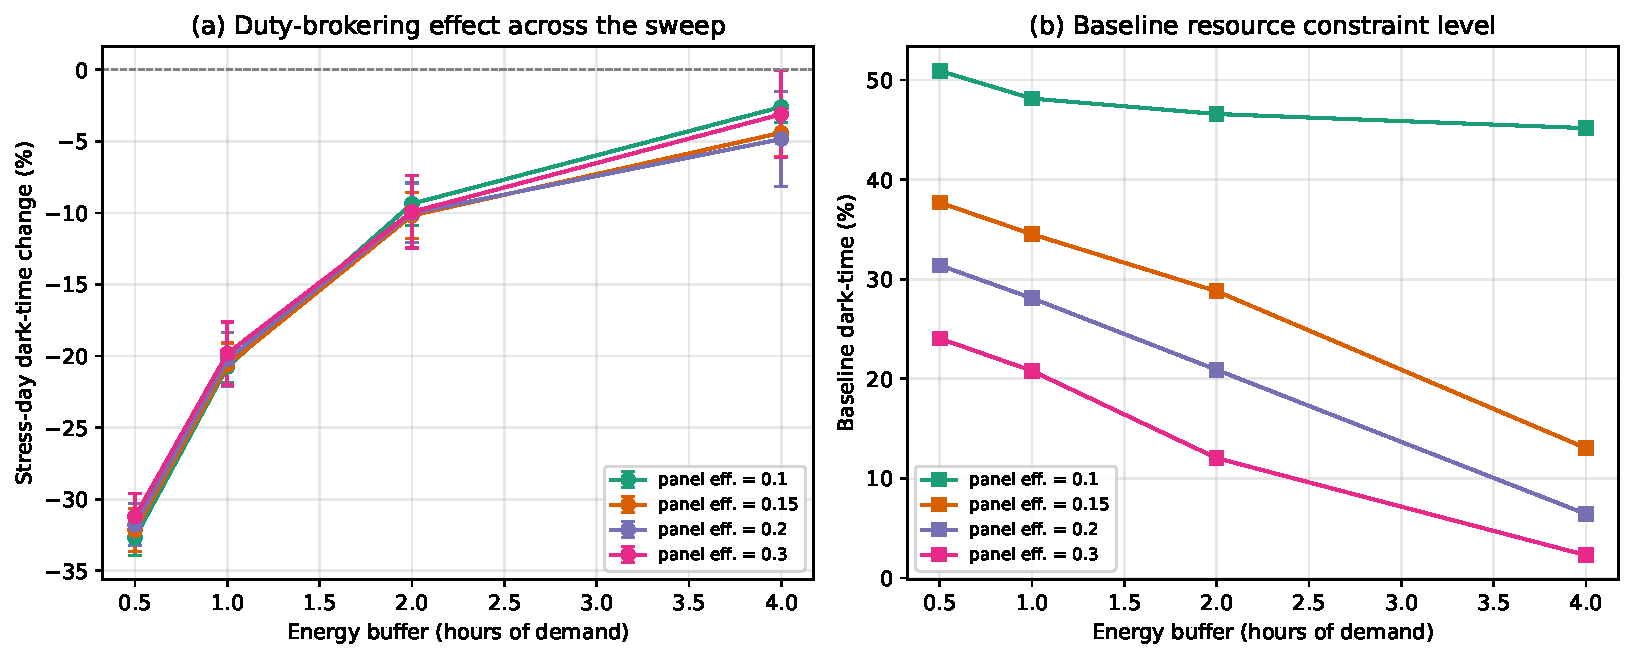
\includegraphics[width=0.95\fulllength]{fig_sweep.pdf}
\end{adjustwidth}
\caption{(\textbf{a}) Duty-brokering's effect on stress-day (monsoon-correlated) dark-time across the full sensitivity sweep, mean $\pm$ standard deviation over 50 seeds per point. The effect is large and statistically clear at resource-constrained settings (small buffer, low panel efficiency) and shrinks toward the noise floor as the system becomes comfortably over-provisioned. (\textbf{b}) The corresponding baseline resource-constraint level (percentage of all simulated minutes the baseline system is dark), shown to make clear why the effect shrinks at generously provisioned settings: a system that rarely fails has little for brokering to fix.\label{fig:sweep}}
\end{figure}

The mechanism driving the effect was non-obvious at design time: even on fully solar-correlated storm days, independently-triggered piezoelectric harvesting events create enough node-to-node buffer asymmetry for brokering to remain useful, rather than the simpler expectation that a fully-correlated storm would leave all nodes equally dark. This is reflected in the stress-day column of Table~\ref{tab:sweep}, where the brokering effect is consistently and substantially larger than on non-stress days across every tested setting, not only at one favorable point.

\subsection{Ablation: Removing the One Unvalidated Model Component}

Setting the flow-harvester placeholder to exactly zero across eight representative grid points (panel efficiency $\in\{0.15,0.20\}$, all four buffer values, 50 seeds each, 400 further seeded runs) left the brokering effect essentially unchanged. Table~\ref{tab:ablation} compares the stress-day effect with and without the placeholder; every ablated value falls within the original run's reported uncertainty, confirming that the headline finding does not depend on the one model component that had no empirical grounding at the time of the original sweep.

\begin{table}[H]
\caption{Ablation: stress-day dark-time reduction with the fabricated flow-harvester placeholder present versus set to exactly zero, eight representative grid points, 50 seeds each.\label{tab:ablation}}
\begin{tabularx}{\textwidth}{CCCC}
\toprule
\textbf{Panel Eff.} & \textbf{Buffer (h)} & \textbf{Stress $\Delta$, with Flow (Placeholder)} & \textbf{Stress $\Delta$, Flow $=$ 0 (Ablated)} \\
\midrule
0.15 & 0.5 & $-32.16\pm1.48\%$ & $-31.97\pm1.47\%$ \\
0.15 & 1.0 & $-20.62\pm1.53\%$ & $-20.17\pm1.85\%$ \\
0.15 & 2.0 & $-10.18\pm1.61\%$ & $-9.60\pm1.72\%$ \\
0.15 & 4.0 & $-4.40\pm1.67\%$ & $-4.26\pm1.98\%$ \\
0.20 & 0.5 & $-31.79\pm1.46\%$ & $-31.51\pm1.55\%$ \\
0.20 & 1.0 & $-20.25\pm1.87\%$ & $-19.90\pm1.98\%$ \\
0.20 & 2.0 & $-10.01\pm2.04\%$ & $-9.87\pm2.07\%$ \\
0.20 & 4.0 & $-4.84\pm3.30\%$ & $-4.64\pm2.41\%$ \\
\bottomrule
\end{tabularx}
\end{table}

\subsection{Flow-Harvester Viability: A Literature-Grounded, Real-Rainfall-Driven Result}
\label{sec:flow-result}

A subsequent, literature-grounded replacement for the flow-harvester placeholder was constructed, driven by real hourly rainfall at the actual highland corridor site (NASA POWER) and a power--velocity curve fitted from two real measured points in a published microturbine characterization study~\cite{ref66} (125~$\mu$W at 0.5~m/s and 5.1~mW at 2.0~m/s). The fitted exponent, 2.68, lies close to the theoretical $v^3$ scaling expected for kinetic turbines, which we take as a sanity check that these are physically consistent measurements rather than noise. Under a disclosed, rational-method runoff model with a concentrated 50~mm~$\times$~50~mm outlet channel, the catchment geometry at which the implied channel velocity stayed within the literature's tested range (1{,}000--2{,}000~m$^2$) predicted the harvester would be active for under 1\% of the year, producing sub-milliwatt power even when active (Table~\ref{tab:flow}). Larger, still-plausible catchment areas produced larger power figures only by extrapolating the fitted curve far beyond its validated velocity range (implied velocities up to 7.6~m/s against a 2.0~m/s upper test limit) and are not reported as credible predictions.

\begin{table}[H]
\caption{Modeled flow-harvester activity under a real rainfall record (Cameron Highlands, 2025) as a function of assumed catchment area, holding channel geometry fixed at 50~mm~$\times$~50~mm. Rows at or above 5{,}000~m$^2$ require extrapolating the fitted power--velocity curve beyond its literature-validated range and are not reported as credible.\label{tab:flow}}
\begin{tabularx}{\textwidth}{CCCCC}
\toprule
\textbf{Catchment (m\boldmath{$^2$})} & \textbf{Active Hours/Year} & \textbf{\% of Year} & \textbf{Mean Power (mW)} & \textbf{Within Tested Velocity Range?} \\
\midrule
500 & 0 & 0.00\% & --- & --- (never reaches cut-in) \\
1{,}000 & 13 & 0.15\% & 0.224 & Yes \\
2{,}000 & 85 & 0.97\% & 0.450 & Yes (peak $\approx$1.5~m/s) \\
5{,}000 & 414 & 4.73\% & 1.402 & \textbf{No --- extrapolated} \\
10{,}000 & 1{,}031 & 11.77\% & 3.803 & \textbf{No --- extrapolated} \\
20{,}000 & 1{,}897 & 21.66\% & 13.365 & \textbf{No --- extrapolated} \\
\bottomrule
\end{tabularx}
\end{table}

This is an unfavorable, quantified result for this specific design component, reported as such rather than adjusted until favorable: at a plausible highway cut-slope catchment size, the flow harvester, as originally conceived, would contribute usable power only during rare, brief windows, not as a reliable complementary source.

\subsection{Real-Data Cross-Checks}
\label{sec:cross-check}

Real paired hourly solar and precipitation data at the actual highland corridor site (NASA POWER) showed a moderate negative correlation between daily rainfall and daily peak solar irradiance ($r = -0.454$, $n = 365$ days), with the wettest-quartile days averaging 15.9\% lower peak solar than the driest quartile, and November showing both the highest mean rainfall and the lowest mean peak solar of any month --- independently matching a solar-only-derived monsoon-suppression signature obtained separately from the Kuala Lumpur dataset. The same reanalysis data, however, returned byte-identical values across three real coordinates spanning a 35~km stretch of the actual highway corridor (Cameron Highlands, Ringlet, and Simpang Pulai), confirming that this data product's native resolution of approximately 1$^\circ$ ($\sim$100~km) cannot resolve the within-corridor spatial decorrelation this paper's correlation-structure assumption requires. This specific question --- whether storm cells genuinely decorrelate at the 10--20~km node spacing the design assumes --- remains open pending ground-station data.

Cross-checking four independently documented, precisely dated real Malaysian landslide incidents against real weather data on their actual dates produced a mixed, informative result, summarized in Table~\ref{tab:events}. One event (6 January 2025, Cameron Highlands) showed a clean same-day match to the predicted high-rain/low-solar signature, with rainfall in the 95.6th percentile of its year and solar in the 11.8th percentile, on the actual reported date of a rain-triggered landslide. A second (21 September 2024, Cameron Highlands) showed no same-day match but a plausible antecedent, cumulative-rainfall pattern, with the darkest day in the surrounding two-month window occurring four days prior. The deadliest event in the set, the Batang Kali campsite landslide of 16 December 2022 (31 deaths), failed on a comparatively sunny day (91.8th percentile peak solar) three days after an extreme dark-and-wet signature (1.6th percentile solar, 91.8th percentile rainfall), consistent with the responsible agency's own stated cause of delayed subsurface saturation. The fourth event (21 May 2011, Hulu Langat, 16 deaths) showed no clear signature match in either direction on the event day or in the preceding days.

\begin{table}[H]
\caption{Real weather conditions on four independently documented, precisely dated Malaysian landslide events, compared to the predicted high-rain/low-solar hazard signature.\label{tab:events}}
\begin{adjustwidth}{-\extralength}{0cm}
\begin{tabularx}{\fulllength}{CCCCC}
\toprule
\textbf{Event} & \textbf{Date} & \textbf{Deaths} & \textbf{Same-Day Signature Match} & \textbf{Notes} \\
\midrule
Cameron Highlands & 6 Jan 2025 & 0 & Clean match (95.6th pctl.\ rain, 11.8th pctl.\ solar) & Explicitly rain-triggered per news reports \\
Cameron Highlands & 21 Sep 2024 & 0 & No same-day match & Darkest day of 2-month window 4 days prior \\
Batang Kali & 16 Dec 2022 & 31 & No same-day match (sunny day) & Extreme dark/wet signature 3 days prior; agency cited delayed subsurface saturation \\
Hulu Langat & 21 May 2011 & 16 & No clear match & Moderate conditions throughout \\
\bottomrule
\end{tabularx}
\end{adjustwidth}
\end{table}

\begin{figure}[H]
\centering
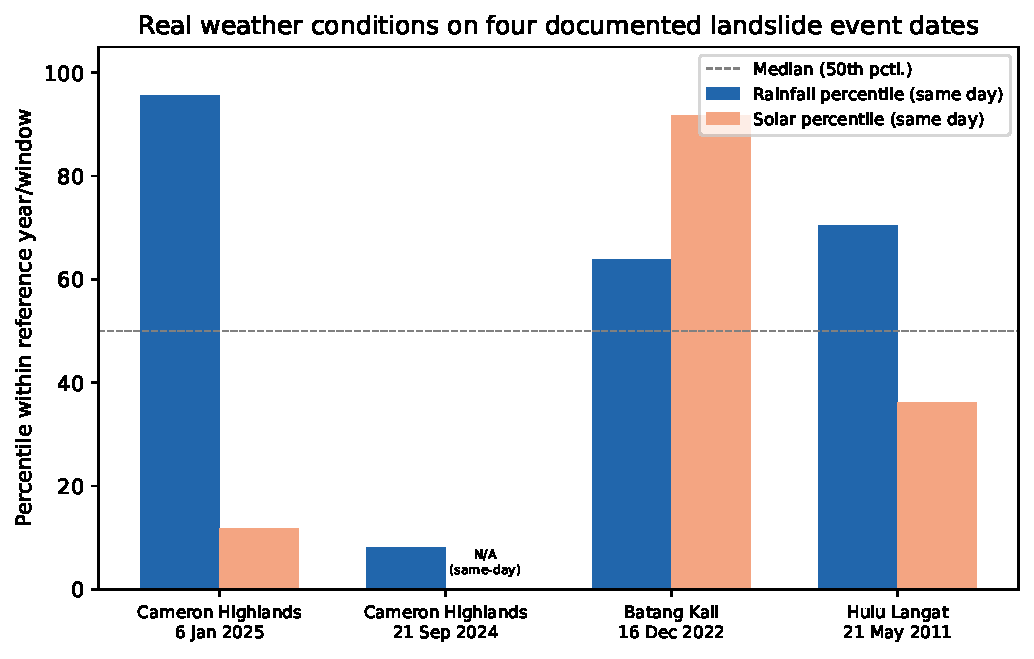
\includegraphics[width=0.75\textwidth]{fig_events.pdf}
\caption{Same-day rainfall and solar-irradiance percentiles (relative to each event's reference year or surrounding window) on the four real, documented landslide event dates cross-checked in this study. The Cameron Highlands (6 January 2025) event shows a clean match to the predicted hazard signature; the Batang Kali event (the deadliest in the set) does not match on the event day itself, consistent with its delayed, cumulative-saturation failure mechanism discussed in Section~\ref{sec:cross-check}. The September 2024 event's same-day solar percentile is not shown because the cross-check for that event (Section~\ref{sec:cross-check}) characterizes it via an antecedent multi-day window rather than a single-day value.\label{fig:events}}
\end{figure}

This heterogeneity, from a sample of four, supports a design conclusion rather than a statistical one. A purely weather-coupled harvesting design would have been at its most relaxed state at exactly the moment the deadliest event in this set actually failed --- a direct, data-derived argument for ground-movement-coupled (piezoelectric) rather than weather-coupled harvesting as the primary design element, independent of the aggregate correlation statistics that originally motivated it.

\section{Discussion}
\label{sec:discussion}

\subsection{What This Process Revised in the Original Design}

The flow-harvester component, present in the design as originally conceived (Section~\ref{sec:design}), is downgraded to a rare-event supplement rather than a core element following the result in Section~\ref{sec:flow-result} --- a revision produced directly by testing the design against real data rather than retained on the strength of the original rationale alone. The piezoelectric component's justification is correspondingly strengthened by the event-level finding in Section~\ref{sec:cross-check}, independent of the aggregate correlation statistics that motivated it originally. We consider this revision process, in which real data was used to challenge rather than merely illustrate the design, to be as important a contribution of this paper as the quantitative results themselves.

\subsection{Internal Validity}
\label{sec:internal-validity}

Two implementation errors were identified and corrected during this work before any result was reported. First, an uncontrolled random-number confound initially let the baseline and treatment conditions draw from different random environments, inflating the apparent treatment effect; this was corrected by seeding two independent random-number streams --- one for environmental stochasticity, shared identically between conditions, and one for brokering-link outcomes, used only by the treatment condition --- rather than a single continuously advancing stream. Second, a day-boundary indexing error caused a thirty-minute brokering hand-off to become, in some cases, effectively permanent, because the per-day timestep index used to check hand-off expiry was reset to zero at the start of each simulated day while the hand-off's expiry timestamp was not. Both errors are reported here, rather than silently corrected, as part of the verification standard applied throughout this study --- including to its own simulation code, not only to the cited literature.

\subsection{External Validity}

This study uses a single-site solar driver (Kuala Lumpur) applied to a hypothetical five-node corridor with an assumed, not measured, spatial correlation structure; an assumed panel and buffer sizing, swept rather than calibrated; and, following Section~\ref{sec:flow-result}, a flow-harvester component now understood to be largely non-viable as originally conceived. The simulation demonstrates that the proposed algorithm is implementable and produces a mechanistically traceable, statistically robust effect under a stated and partly real-data-grounded set of assumptions. It does not demonstrate that effect's magnitude at an actual highway cut-slope deployment, and should not be read as doing so.

\subsection{Source and Data Verification}
\label{sec:verification}

Venue-quality screening during the literature review identified one source~\cite{ref66} that could not be independently re-verified within the scope of this study after an attempt to access its full text was blocked (HTTP 403) on two separate occasions; this source is cited only for its reported power--velocity anchor points (Section~\ref{sec:flow-result}), which are also independently consistent with the theoretical $v^3$ kinetic-turbine scaling, and not for any claim requiring trust in unverified surrounding content. One further source identified during screening, published by a venue with documented, unrelated large-scale peer-review integrity concerns disclosed by its publisher in 2023, was excluded from this manuscript's citation set entirely rather than cited with a caveat, since the specific article's standing could not be confirmed. All datasets used for simulation input (Section~\ref{sec:methods}) were confirmed to exist via direct retrieval before use, and their license terms are stated there.

\subsection{Required Steps Before Deployment}

Closing the gap between this preliminary feasibility study and a deployment-ready system requires, at minimum: real multi-site weather data at a resolution capable of resolving the within-corridor spatial-correlation assumption (ground-station data, not satellite reanalysis, per Section~\ref{sec:cross-check}); a real flow-harvester characterization under sediment-laden, intermittent field conditions, should that component be pursued further; calibrated, rather than assumed, structural constants for panel efficiency, buffer sizing, and movement-trigger probabilities; and the hardware-in-the-loop and physical-prototype validation stages the reference architecture itself used~\cite{ref101}, extended to the multi-node configuration this paper's algorithm requires. None of these have yet been carried out, and we make no claim that they have.

\section{Conclusions}
\label{sec:conclusion}

This paper proposes and computationally tests an extension of a validated single-node IoT-microgrid architecture to a deployment class --- off-grid landslide-monitoring swarms on Malaysian highway cut-slopes --- where the original architecture's utility-backup assumption does not hold. A 50-seed Monte Carlo simulation, driven by real solar and piezoelectric harvester data, shows that corridor-wide duty-brokering produces a statistically robust reduction in sensing downtime concentrated specifically on the correlated storm conditions the design targets, and that this finding is not an artifact of its one unvalidated model component. Cross-checking the design's premises against real weather data and real documented landslide incidents produced genuinely mixed evidence that nonetheless motivated a concrete, favorable revision to the design, strengthening the case for ground-movement-coupled harvesting, and a concrete, unfavorable one, downgrading the flow-harvester component after finding it viable for well under 1\% of the year under realistic geometry. The result is a preliminary feasibility study, not a field validation; we have specified the real-world data and hardware-in-the-loop work still required to close that gap, and we have not performed it.

\vspace{6pt}

\authorcontributions{Conceptualization, S.K.\ and S.Y.; methodology, S.K.; software, S.K.; formal analysis, S.K.; investigation, S.K.\ and S.Y.; data curation, S.K.; writing---original draft preparation, S.K.; writing---review and editing, S.K.\ and S.Y.; supervision, S.Y. All authors have read and agreed to the published version of the manuscript.}

\funding{This research received no external funding.}

\institutionalreview{Not applicable. This study involved no human subjects, animal subjects, or personally identifiable data; all datasets used are publicly available environmental and laboratory measurement data.}

\informedconsent{Not applicable.}

\dataavailability{Datasets used: Kuala Lumpur solar irradiance (Mendeley Data, DOI: 10.17632/bgch4tw79k.1, CC BY 4.0); piezoelectric harvester characterization (Mendeley Data, DOI: 10.17632/y4cmrsdv9f.1, CC BY 4.0); NASA POWER hourly reanalysis data (publicly available via the POWER Project application programming interface, power.larc.nasa.gov, no registration required). Simulation code supporting the findings of this study is available from the corresponding author upon reasonable request.}

\acknowledgments{During the preparation of this manuscript, the authors used AI-assisted tools for literature search and screening, source verification, simulation code implementation, and manuscript drafting. All quantitative claims were independently computed by executing the described code against the cited datasets rather than generated from model memory; two implementation errors identified during this process are disclosed in Section~\ref{sec:internal-validity}. The authors have reviewed and edited the output and take full responsibility for the content of this publication.}

\conflictsofinterest{The authors declare no conflicts of interest. The funders had no role in the design of the study; in the collection, analyses, or interpretation of data; in the writing of the manuscript; or in the decision to publish the results.}

\abbreviations{Abbreviations}{%
The following abbreviations are used in this manuscript:\\
\noindent
\begin{tabular}{@{}ll}
IoT & Internet of Things\\
HIL & Hardware-in-the-Loop\\
PHIL & Power Hardware-in-the-Loop\\
WSN & Wireless Sensor Network\\
LPWAN & Low-Power Wide-Area Network\\
LoRaWAN & Long Range Wide Area Network\\
PDR & Packet Delivery Ratio\\
GHI & Global Horizontal Irradiance\\
P2P & Peer-to-Peer\\
JKR & Jabatan Kerja Raya (Public Works Department, Malaysia)\\
PRISMA & Preferred Reporting Items for Systematic Reviews and Meta-Analyses
\end{tabular}
}

\begin{adjustwidth}{-\extralength}{0cm}
\reftitle{References}

\begin{thebibliography}{150}
\bibitem{ref1}
El Houssaini et al. (2022). Location-Aware IoT-Enabled WSNs for Landslide Early Warning. \textit{Electronics}. Available online: https://doi.org/10.3390/electronics11233971 (accessed on 17 October 2026).
\bibitem{ref2}
Giri et al. (2019). WSN System for Landslide Monitoring and Warning. \textit{IEEE Trans. Instrum. Meas.}. Available online: https://doi.org/10.1109/tim.2018.2861999 (accessed on 17 October 2026).
\bibitem{ref3}
Rani et al. (2025). IoT-Enabled Real-Time Landslide Monitoring using Waterbody Sensors. \textit{ICTMIM 2025}. Available online: https://doi.org/10.1109/ictmim65579.2025.10988011 (accessed on 17 October 2026).
\bibitem{ref4}
Gowtham et al. (2026). Low-Power LoRaWAN IoT Landslide EWS with Random Forest. \textit{ICAISS 2026}. Available online: https://doi.org/10.1109/icaiss68683.2026.11525861 (accessed on 17 October 2026).
\bibitem{ref5}
Amirthavarshini et al. (2025). Harnessing LoRa for Real-Time Landslide Monitoring in Kerala. \textit{Geoscience Frontiers}. Available online: https://doi.org/10.1016/j.gsf.2025.102242 (accessed on 17 October 2026).
\bibitem{ref6}
Souza et al. (2022). IoT-Based System for Landslides Warnings Using Real Time Slope Monitoring. \textit{COTB'22}. Available online: https://doi.org/10.14210/cotb.v13.p126-133 (accessed on 17 October 2026).
\bibitem{ref7}
D. J. et al. (2025). I-ELWS: IoT Driven Early Landslide Warning System. \textit{ETNCC 2025}. Available online: https://doi.org/10.1109/etncc66224.2025.11299651 (accessed on 17 October 2026).
\bibitem{ref8}
P. C. et al. (2021). Real-time landslide EWS through low cost soil and rainfall sensors. \textit{Materials Today: Proceedings}. Available online: https://doi.org/10.1016/j.matpr.2021.02.456 (accessed on 17 October 2026).
\bibitem{ref9}
Chaulya et al. (2024). Landslide monitoring and prediction system using geosensors and WSN. \textit{Discover Geoscience}. Available online: https://doi.org/10.1007/s44288-024-00007-3 (accessed on 17 October 2026).
\bibitem{ref10}
Susanto et al. (2024). Landslide Monitoring and Warning System Based on WSN. \textit{ELKHA}. Available online: https://doi.org/10.26418/elkha.v16i2.83489 (accessed on 17 October 2026).
\bibitem{ref11}
Thein et al. (2020). Real-Time Monitoring and EWS for Landslide Preventing in Myanmar. \textit{GCCE 2020}. Available online: https://doi.org/10.1109/gcce50665.2020.9291809 (accessed on 17 October 2026).
\bibitem{ref12}
Ramesh (2009). Real-Time WSN for Landslide Detection. \textit{SensorComm 2009}. Available online: https://doi.org/10.1109/sensorcomm.2009.67 (accessed on 17 October 2026).
\bibitem{ref13}
Devi (2025). Developing a Low-Cost Landslide EWS using IoT and Sensor Networks. \textit{ICSCSS 2025}. Available online: https://doi.org/10.1109/icscss64956.2025.11501071 (accessed on 17 October 2026).
\bibitem{ref14}
Gamperl et al. (2021). IoT Geosensor Network for Cost-Effective LEWS (Inform@Risk, Colombia). \textit{Sensors}. Available online: https://doi.org/10.3390/s21082609 (accessed on 17 October 2026).
\bibitem{ref15}
Mahfudh et al. (2026). Low-Cost IoT-Based Landslide EWS. \textit{CENTIVE Proceedings}. Available online: https://doi.org/10.20895/centive.v2025i1.562 (accessed on 17 October 2026).
\bibitem{ref16}
Rawat et al. (2024). LANDSLIDE MONITOR: a real-time landslide monitoring system. \textit{Environ. Earth Sci.}. Available online: https://doi.org/10.1007/s12665-024-11526-0 (accessed on 17 October 2026).
\bibitem{ref17}
Galley et al. (2017). WSN Based Landslide Detection and EWS. \textit{Zorig Melong}. Available online: https://doi.org/10.17102/zmv3.i1.006 (accessed on 17 October 2026).
\bibitem{ref18}
Abraham et al. (2020). IoT-Based Geotechnical Monitoring, Darjeeling Himalayas. \textit{Sensors}. Available online: https://doi.org/10.3390/s20092611 (accessed on 17 October 2026).
\bibitem{ref19}
Das et al. (2020). Real-Time Threshold-based Landslide Prediction using WSN. \textit{ICCE-Taiwan 2020}. Available online: https://doi.org/10.1109/icce-taiwan49838.2020.9258181 (accessed on 17 October 2026).
\bibitem{ref20}
Ramesh et al. (2017). WSNs for Early Warning of Landslides: Decade Long Deployment. Available online: https://doi.org/10.1007/978-3-319-53487-9\_4 (accessed on 17 October 2026).
\bibitem{ref21}
Ali et al. (2012). Development of WSN for slope monitoring (Hulu Langat, MALAYSIA, 2011 landslide, 16 fatalities). \textit{ICIAS 2012}. Available online: https://doi.org/10.1109/icias.2012.6306203 (accessed on 17 October 2026).
\bibitem{ref22}
Ragnoli et al. (2023). WSN-Based Rockfall and Landslide Monitoring Systems: A Review. \textit{Sensors}. Available online: https://doi.org/10.3390/s23167278 (accessed on 17 October 2026).
\bibitem{ref23}
Bagwari et al. (2021). Low-Cost Sensor and LoRaWAN Opportunities for Landslide Monitoring: A Review. \textit{IEEE Access}. Available online: https://doi.org/10.1109/access.2021.3137841 (accessed on 17 October 2026).
\bibitem{ref24}
Jeong et al. (2019). Effectiveness of a WSN System for Landslide Monitoring (Seoul). \textit{IEEE Access}. Available online: https://doi.org/10.1109/access.2019.2960570 (accessed on 17 October 2026).
\bibitem{ref25}
Marino et al. (2023). IoT-Based Low-Cost Sensor Network for Hydrological Monitoring of Landslide-Prone Areas. \textit{Sensors}. Available online: https://doi.org/10.3390/s23042299 (accessed on 17 October 2026).
\bibitem{ref26}
Debnath et al. (2025). Smart IoT-Based Distributed System for Remote Detection of Slope Movements (highway embankments). \textit{ICNC 2025}. Available online: https://doi.org/10.1109/icnc64010.2025.10993553 (accessed on 17 October 2026).
\bibitem{ref27}
Ahmed et al. (2016). Real-time monitoring of partially stable slopes using WSN. \textit{IC-GET 2016}. Available online: https://doi.org/10.1109/get.2016.7916638 (accessed on 17 October 2026).
\bibitem{ref28}
Vu et al. (2018). WSN in landslide monitoring system with remote data management. \textit{Measurement}. Available online: https://doi.org/10.1016/j.measurement.2018.01.002 (accessed on 17 October 2026).
\bibitem{ref29}
Kumar M. et al. (2022). Accurate IoT Based Slope Instability Sensing System for Landslide Detection. \textit{IEEE Sensors J.}. Available online: https://doi.org/10.1109/jsen.2022.3189903 (accessed on 17 October 2026).
\bibitem{ref30}
Joshi et al. (2023). WSN-Based Smart Landslide Monitoring Device (SMARTMODE). \textit{IEEE Trans. Instrum. Meas.}. Available online: https://doi.org/10.1109/tim.2023.3269746 (accessed on 17 October 2026).
\bibitem{ref32}
Piciullo et al. (2017). Threshold-based regional EW model for rainfall-induced landslides. \textit{Landslides}. Available online: https://doi.org/10.1007/s10346-016-0750-2 (accessed on 17 October 2026).
\bibitem{ref33}
Liu et al. (2024). Regional EW model based on slope unit, Chongqing. \textit{Engineering Geology}. Available online: https://doi.org/10.1016/j.enggeo.2024.107464 (accessed on 17 October 2026).
\bibitem{ref34}
Dou et al. (2024). Regional dynamic EW model, Fujian. \textit{Geomatics, Nat. Hazards and Risk}. Available online: https://doi.org/10.1080/19475705.2024.2435510 (accessed on 17 October 2026).
\bibitem{ref35}
Guzzetti et al. (2024). Landslide predictions through combined rainfall threshold models. \textit{Landslides}. Available online: https://doi.org/10.1007/s10346-024-02340-7 (accessed on 17 October 2026).
\bibitem{ref36}
Huang et al. (2022). Regional rainfall-induced landslide hazard warning based on susceptibility mapping. \textit{Geomorphology}. Available online: https://doi.org/10.1016/j.geomorph.2022.108236 (accessed on 17 October 2026).
\bibitem{ref37}
Zhang et al. (2026). Dynamic EW Model Coupling Slope Units and Rainfall Thresholds, Jinyang. \textit{Geosciences}. Available online: https://doi.org/10.3390/geosciences16090367 (accessed on 17 October 2026).
\bibitem{ref38}
Cao et al. (2022). Hourly shallow landslide warning model combining susceptibility and rainfall threshold. \textit{J. Mountain Sci.}. Available online: https://doi.org/10.1007/s11629-022-7370-1 (accessed on 17 October 2026).
\bibitem{ref39}
Song et al. (2025). Refined meteorological EW based on temporal probability model. \textit{Chinese J. Rock Mech. Eng.}. Available online: https://doi.org/10.3724/1000-6915.jrme.2024.0805 (accessed on 17 October 2026).
\bibitem{ref40}
Wang et al. (2026). Dynamic EW model based on refined threshold analysis, Tanjiawan. \textit{PLOS One}. Available online: https://doi.org/10.1371/journal.pone.0339689 (accessed on 17 October 2026).
\bibitem{ref41}
Zhan et al. (2022). EW model and model test verification of rainfall-induced shallow landslide. \textit{Bull. Eng. Geol. Environ.}. Available online: https://doi.org/10.1007/s10064-022-02827-4 (accessed on 17 October 2026).
\bibitem{ref42}
Nocentini et al. (2023). Optimization of rainfall thresholds through false alarm reduction. \textit{Landslides}. Available online: https://doi.org/10.1007/s10346-023-02176-7 (accessed on 17 October 2026).
\bibitem{ref43}
Sun et al. (2024). Probabilistic thresholds for regional rainfall induced landslides. \textit{Computers and Geotechnics}. Available online: https://doi.org/10.1016/j.compgeo.2023.106040 (accessed on 17 October 2026).
\bibitem{ref44}
Naidu et al. (2017). EWS for shallow landslides using rainfall threshold and slope stability analysis. \textit{Geoscience Frontiers}. Available online: https://doi.org/10.1016/j.gsf.2017.10.008 (accessed on 17 October 2026).
\bibitem{ref45}
Dou et al. (2023). Rainfall EW threshold and spatial distribution in China. \textit{Rock Mechanics Bulletin}. Available online: https://doi.org/10.1016/j.rockmb.2023.100056 (accessed on 17 October 2026).
\bibitem{ref46}
Dixit et al. (2024). Numerical-model-derived I-D thresholds for debris flows, Himalayan catchment. \textit{NHESS}. Available online: https://doi.org/10.5194/nhess-24-465-2024 (accessed on 17 October 2026).
\bibitem{ref47}
Lee et al. (2021). Optimal rainfall thresholds for LEWS, Chuncheon, Korea. \textit{Landslides}. Available online: https://doi.org/10.1007/s10346-020-01603-3 (accessed on 17 October 2026).
\bibitem{ref48}
Wang et al. (2026). Physical-based rainfall landslide prediction model from slope-unit I-D curves. \textit{NHESS}. Available online: https://doi.org/10.5194/nhess-26-2367-2026 (accessed on 17 October 2026).
\bibitem{ref49}
Sarkar et al. (2023). Event-duration rainfall threshold model, Uttarkashi, Himalayas. \textit{Int. J. Earth Sci.}. Available online: https://doi.org/10.1007/s00531-023-02337-y (accessed on 17 October 2026).
\bibitem{ref50}
Li et al. (2026). Sustained Self-Powered Real-Time Vibration Monitoring via Nonlinear Harvesting. \textit{Advanced Science}. Available online: https://doi.org/10.1002/advs.76967 (accessed on 17 October 2026).
\bibitem{ref51}
Rubeš et al. (2021). Self-powered wireless vibration sensor node using vibration energy harvester. \textit{Mech. Syst. Signal Process.}. Available online: https://doi.org/10.1016/j.ymssp.2021.107890 (accessed on 17 October 2026).
\bibitem{ref52}
Izhar et al. (2023). Hybrid acoustic, vibration, and wind energy harvester for self-powered WSN. \textit{Energy Conversion and Management}. Available online: https://doi.org/10.1016/j.enconman.2022.116635 (accessed on 17 October 2026).
\bibitem{ref53}
Wang et al. (2024). Sensor-enabled piezoelectric geocable–geogrid for slope rehabilitation and monitoring. \textit{Engineering Geology}. Available online: https://doi.org/10.1016/j.enggeo.2024.107780 (accessed on 17 October 2026).
\bibitem{ref54}
Wang et al. (2026). Reinforcement and microseismic monitoring of slopes with self-sensing smart geosynthetic. \textit{Geosynthetics International}. Available online: https://doi.org/10.1680/jgein.25.00212 (accessed on 17 October 2026).
\bibitem{ref55}
Rigo et al. (2024). Piezoelectric Sensors as Energy Harvesters for Ultra Low-Power IoT. \textit{Sensors}. Available online: https://doi.org/10.3390/s24082587 (accessed on 17 October 2026).
\bibitem{ref56}
Wang et al. (2024). Self-sustained/self-wakeup wireless vibration sensors, hybrid harvesting. \textit{Applied Energy}. Available online: https://doi.org/10.1016/j.apenergy.2023.122207 (accessed on 17 October 2026).
\bibitem{ref57}
Yang et al. (2025). Hybrid multiple-layer piezoelectric-solar harvester for self-powered sensing. \textit{Sustainable Energy Technologies and Assessments}. Available online: https://doi.org/10.1016/j.seta.2024.104157 (accessed on 17 October 2026).
\bibitem{ref58}
Li et al. (2021). Piezoelectric Energy Harvesting: Materials, Structures, Applications. \textit{Small Structures}. Available online: https://doi.org/10.1002/sstr.202100128 (accessed on 17 October 2026).
\bibitem{ref59}
Ng et al. (2005). Sensitivity Analysis and Energy Harvesting for a Self-Powered Piezoelectric Sensor. \textit{J. Intelligent Material Systems and Structures}. Available online: https://doi.org/10.1177/1045389x05053151 (accessed on 17 October 2026).
\bibitem{ref60}
Lo et al. (2022). Self-powered SECE piezoelectric harvesting from shock excitations. \textit{Mech. Syst. Signal Process.}. Available online: https://doi.org/10.1016/j.ymssp.2022.109123 (accessed on 17 October 2026).
\bibitem{ref61}
Biswal et al. (2024). Self-Powered Accelerometer Using Circular Hole Piezo Harvester. \textit{IEEE Sensors Letters}. Available online: https://doi.org/10.1109/lsens.2024.3485540 (accessed on 17 October 2026).
\bibitem{ref62}
Kuang et al. (2021). Strongly coupled piezoelectric harvesters for self-powered condition monitoring. \textit{Energy Conversion and Management}. Available online: https://doi.org/10.1016/j.enconman.2021.114129 (accessed on 17 October 2026).
\bibitem{ref63}
Zou (2023). Piezoelectric self-powered wireless sensor in vibration environment monitoring. \textit{Results in Engineering}. Available online: https://doi.org/10.1016/j.rineng.2023.101492 (accessed on 17 October 2026).
\bibitem{ref64}
Das Mahapatra et al. (2021). Piezoelectric Materials for Energy Harvesting and Sensing: Roadmap. \textit{Advanced Science}. Available online: https://doi.org/10.1002/advs.202100864 (accessed on 17 October 2026).
\bibitem{ref66}
Lepipas et al. (2024). Miniature water flow harvester, Savonius-type microturbine. \textit{Smart Materials and Structures}. Available online: https://doi.org/10.1088/1361-665x/ad1c3f (accessed on 17 October 2026).
\bibitem{ref67}
Guiffard et al. (2021). Self-powered wireless sensor with flexible aero-piezoelectric harvester. \textit{Renewable Energy}. Available online: https://doi.org/10.1016/j.renene.2021.11.113 (accessed on 17 October 2026).
\bibitem{ref68}
Zhang et al. (2024). Triboelectric-EM hybrid generator, Savonius flapping wing, low-velocity water flow. \textit{Applied Energy}. Available online: https://doi.org/10.1016/j.apenergy.2023.122512 (accessed on 17 October 2026).
\bibitem{ref69}
Rahman et al. (2025). Survey of flow-based energy harvesters for sustainable WSN nodes. \textit{J. Renewable and Sustainable Energy}. Available online: https://doi.org/10.1063/5.0237597 (accessed on 17 October 2026).
\bibitem{ref70}
Zhao et al. (2021). Hydrokinetic piezoelectric harvesting by wake-induced vibration. \textit{Energy}. Available online: https://doi.org/10.1016/j.energy.2020.119722 (accessed on 17 October 2026).
\bibitem{ref71}
Kamenar et al. (2016). Harvesting river flow energy for WSN technology (GOLDFISH project). \textit{Microsystem Technologies}. Available online: https://doi.org/10.1007/s00542-015-2778-y (accessed on 17 October 2026).
\bibitem{ref72}
Li et al. (2022). Self-powered wireless water-monitoring sensor, electromagnetic-pendulum harvester. \textit{Energy}. Available online: https://doi.org/10.1016/j.energy.2022.123883 (accessed on 17 October 2026).
\bibitem{ref73}
Vijayaregunathan et al. (2024). Harvesting hydraulic energy for self-sustainable IoT flow measurement. \textit{Energy Sources Part A}. Available online: https://doi.org/10.1080/15567036.2024.2334922 (accessed on 17 October 2026).
\bibitem{ref74}
Yunus et al. (2026). Design of a Wireless Sensor Node Powered by Kinetic Energy Harvesters. \textit{Applied Research}. Available online: https://doi.org/10.1002/appl.70124 (accessed on 17 October 2026).
\bibitem{ref75}
Zhou et al. (2026). Small-scale water energy harvesting for sustainably-powered distributed electronics. \textit{Communications Materials}. Available online: https://doi.org/10.1038/s43246-026-01137-6 (accessed on 17 October 2026).
\bibitem{ref76}
Sarker et al. (2024). Micro energy harvesting for IoT platform: Review. \textit{Heliyon}. Available online: https://doi.org/10.1016/j.heliyon.2024.e27778 (accessed on 17 October 2026).
\bibitem{ref77}
Hafizh et al. (2023). Vortex-induced-vibration self-tunable airfoil piezoelectric harvester for underwater sensing. \textit{Ocean Engineering}. Available online: https://doi.org/10.1016/j.oceaneng.2022.113467 (accessed on 17 October 2026).
\bibitem{ref78}
Azevedo et al. (2012). Energy harvesting from wind and water for autonomous WSN nodes. \textit{IET Circuits Devices Syst.}. Available online: https://doi.org/10.1049/iet-cds.2011.0287 (accessed on 17 October 2026).
\bibitem{ref79}
Williams et al. (2021). Survey of Energy Harvesting Technologies for WSNs. \textit{IEEE Access}. Available online: https://doi.org/10.1109/access.2021.3083697 (accessed on 17 October 2026).
\bibitem{ref81}
Ragnoli et al. (2020). Autonomous Low-Power LoRa-Based Flood-Monitoring System. \textit{J. Low Power Electronics and Applications}. Available online: https://doi.org/10.3390/jlpea10020015 (accessed on 17 October 2026).
\bibitem{ref82}
Tsakmakis et al. (2022). Adaptive LoRaWAN MAC Protocol for Event Detection Applications. \textit{Sensors}. Available online: https://doi.org/10.3390/s22093538 (accessed on 17 October 2026).
\bibitem{ref83}
Pan et al. (2021). UAV-Aided Emergency Environmental Monitoring, LoRa Mesh. \textit{IEEE IoT Journal}. Available online: https://doi.org/10.1109/jiot.2021.3095494 (accessed on 17 October 2026).
\bibitem{ref84}
Sendra et al. (2020). LoRaWAN Network for Fire Monitoring in Rural Environments. \textit{Electronics}. Available online: https://doi.org/10.3390/electronics9030531 (accessed on 17 October 2026).
\bibitem{ref86}
Ragnoli et al. (2022). LoRa-Based WSN for Rockfall and Landslide Monitoring, Pantelleria Island. \textit{J. Low Power Electronics and Applications}. Available online: https://doi.org/10.3390/jlpea12030047 (accessed on 17 October 2026).
\bibitem{ref87}
Wu et al. (2023). Low-Cost Low-Power LoRa Mesh Network for Large-Scale Environmental Sensing (CottonCandy). \textit{IEEE IoT Journal}. Available online: https://doi.org/10.1109/jiot.2023.3270237 (accessed on 17 October 2026).
\bibitem{ref88}
Finochietto et al. (2022). Reducing Operational Expenses of LoRaWAN-Based IoRT Applications. \textit{Sensors}. Available online: https://doi.org/10.3390/s22207778 (accessed on 17 October 2026).
\bibitem{ref89}
Bagwari et al. (2022). Disaster Monitoring based on IoT and Long Range Assisted Framework. \textit{J. Physics: Conf. Series}. Available online: https://doi.org/10.1088/1742-6596/2327/1/012020 (accessed on 17 October 2026).
\bibitem{ref90}
Ragnoli et al. (2022). Flood monitoring: LoRa-based case study, L'Aquila. \textit{PRIME 2022}. Available online: https://doi.org/10.1109/prime55000.2022.9816747 (accessed on 17 October 2026).
\bibitem{ref91}
Abdul Latiff (2019). Environmental Monitoring System Based on LoRa Technology in Island. \textit{ICSigSys 2019}. Available online: https://doi.org/10.1109/icsigsys.2019.8811066 (accessed on 17 October 2026).
\bibitem{ref92}
Chapungo et al. (2025). LoRaWAN Connectivity Reliability in Remote Rural Areas of Mozambique (source of the ~89\% PDR lossy-link finding used in Phase 3 synthesis). \textit{Sensors}. Available online: https://doi.org/10.3390/s25196027 (accessed on 17 October 2026).
\bibitem{ref93}
Zhao et al. (2023). Forest IoT Using LPWAN, Solar-Powered Micro-Weather Station. \textit{Sensors}. Available online: https://doi.org/10.3390/s23104809 (accessed on 17 October 2026).
\bibitem{ref94}
Tamang et al. (2022). Reliable Low-Latency LoRaWAN Solution for Environmental Monitoring at Major Accident Risk Sites. \textit{Sensors}. Available online: https://doi.org/10.3390/s22062372 (accessed on 17 October 2026).
\bibitem{ref95}
Liya et al. (2026). Energy efficient cyber-physical control of renewable microgrids, edge-AI, blockchain. \textit{Scientific Reports}. Available online: https://doi.org/10.1038/s41598-026-50169-y (accessed on 17 October 2026).
\bibitem{ref96}
Silva et al. (2023). IoT-based EMS for AC microgrids with grid and security constraints. \textit{Applied Energy}. Available online: https://doi.org/10.1016/j.apenergy.2023.120904 (accessed on 17 October 2026).
\bibitem{ref97}
Wu et al. (2024). Microgrids EM considering net-zero energy, IoT digital twin. \textit{Sustainable Energy Technologies and Assessments}. Available online: https://doi.org/10.1016/j.seta.2024.103621 (accessed on 17 October 2026).
\bibitem{ref98}
Cicceri et al. (2023). Deep Learning-Driven Self-Conscious Distributed CPS for Renewable Energy Communities. \textit{Sensors}. Available online: https://doi.org/10.3390/s23094549 (accessed on 17 October 2026).
\bibitem{ref99}
Asef et al. (2023). SIEMS: Secure Intelligent EMS for Industrial IoT Applications. \textit{IEEE Trans. Industrial Informatics}. Available online: https://doi.org/10.1109/tii.2022.3165890 (accessed on 17 October 2026).
\bibitem{ref100}
Tasmant et al. (2025). Review of ML and IoT-based EMS for AC microgrids. \textit{Comput. Electr. Eng.}. Available online: https://doi.org/10.1016/j.compeleceng.2025.110563 (accessed on 17 October 2026).
\bibitem{ref101}
Lee \& Wang (2024). A Cyber-Physical Testbed for IoT Microgrid Design and Validation [PRIMARY REFERENCE PAPER]. \textit{Electronics}. Available online: https://doi.org/10.3390/electronics13071181 (accessed on 17 October 2026).
\bibitem{ref102}
Albarakati et al. (2022). Microgrid energy management and monitoring systems: A comprehensive review. \textit{Frontiers in Energy Research}. Available online: https://doi.org/10.3389/fenrg.2022.1097858 (accessed on 17 October 2026).
\bibitem{ref103}
Xu et al. (2021). Blockchain-based secure energy policy and management of renewable smart microgrids. \textit{Sustainable Cities and Society}. Available online: https://doi.org/10.1016/j.scs.2021.103010 (accessed on 17 October 2026).
\bibitem{ref104}
Sitharthan et al. (2023). Smart microgrid with IoT for energy management (PV/Wind/Piezo hybrid). \textit{Comput. Electr. Eng.}. Available online: https://doi.org/10.1016/j.compeleceng.2022.108556 (accessed on 17 October 2026).
\bibitem{ref105}
Mallala et al. (2025). IoT-enabled community microgrid EM with battery degradation consideration. \textit{J. Energy Storage}. Available online: https://doi.org/10.1016/j.est.2024.114739 (accessed on 17 October 2026).
\bibitem{ref107}
Samanta et al. (2020). IoT-based smart EM in VRFB-integrated bio-solar microgrid. \textit{J. Energy Storage}. Available online: https://doi.org/10.1016/j.est.2020.101967 (accessed on 17 October 2026).
\bibitem{ref108}
Aljafari et al. (2022). Optimization of DC, AC, Hybrid AC/DC Microgrid-Based IoT Systems: A Review. \textit{Energies}. Available online: https://doi.org/10.3390/en15186813 (accessed on 17 October 2026).
\bibitem{ref109}
Sedhom et al. (2021). IoT-based optimal demand side management for smart microgrid. \textit{Int. J. Electrical Power \& Energy Systems}. Available online: https://doi.org/10.1016/j.ijepes.2020.106674 (accessed on 17 October 2026).
\bibitem{ref110}
Zhou et al. (2021). Multi-microgrid EMS: Architecture, Communication, and Scheduling Strategies. \textit{J. Modern Power Systems and Clean Energy}. Available online: https://doi.org/10.35833/mpce.2019.000237 (accessed on 17 October 2026).
\bibitem{ref111}
Ojo et al. (2025). Microgrids' Control Strategies and Real-Time Monitoring Systems: Comprehensive Review. \textit{Energies}. Available online: https://doi.org/10.3390/en18133576 (accessed on 17 October 2026).
\bibitem{ref112}
Alhasnawi et al. (2023). New communication platform for smart EMS using MILP. \textit{Energy Systems}. Available online: https://doi.org/10.1007/s12667-023-00591-2 (accessed on 17 October 2026).
\bibitem{ref113}
Bahbahani et al. (2017). Cooperative Clustering Protocol With Duty Cycling for EH-WSN. \textit{IEEE Trans. Wireless Communications}. Available online: https://doi.org/10.1109/twc.2017.2762674 (accessed on 17 October 2026).
\bibitem{ref114}
Shagari et al. (2020). Heterogeneous Energy and Traffic Aware Sleep-Awake Cluster-Based Routing. \textit{IEEE Access}. Available online: https://doi.org/10.1109/access.2020.2965206 (accessed on 17 October 2026).
\bibitem{ref115}
Ramkumar (2025). Adaptive Duty-Cycled Cooperative Clustering Model for EH-WSN. \textit{CNC 2025}. Available online: https://doi.org/10.1109/cnc68716.2025.11484711 (accessed on 17 October 2026).
\bibitem{ref116}
Liu et al. (2023). DCC-IACJS: bio-inspired duty cycle-based clustering for energy-efficient WSN. \textit{J. King Saud University CIS}. Available online: https://doi.org/10.1016/j.jksuci.2023.01.015 (accessed on 17 October 2026).
\bibitem{ref117}
V. et al. (2025). Energy-Aware MAC Protocols with Load Balancing for Solar-Powered WSN. \textit{ICDSNS 2025}. Available online: https://doi.org/10.1109/icdsns65743.2025.11168589 (accessed on 17 October 2026).
\bibitem{ref118}
Tolani et al. (2023). Energy-Efficient Duty-Cycle Hybrid MAC Protocol for WSN. \textit{Wireless Personal Communications}. Available online: https://doi.org/10.1007/s11277-023-10448-7 (accessed on 17 October 2026).
\bibitem{ref119}
Chauhan et al. (2022). Variable duty cycle aware energy efficient clustering strategy for WSN. \textit{J. Ambient Intelligence and Humanized Computing}. Available online: https://doi.org/10.1007/s12652-022-04363-1 (accessed on 17 October 2026).
\bibitem{ref120}
Gong et al. (2023). Centralized Energy-Efficient Clustering Protocol for WSN. \textit{IEEE Sensors J.}. Available online: https://doi.org/10.1109/jsen.2022.3224180 (accessed on 17 October 2026).
\bibitem{ref121}
Yang et al. (2025). DRL-Driven Workload Offloading for Energy-Efficient Solar-Powered WSN. \textit{ACM CoNEXT Workshop}. Available online: https://doi.org/10.1145/3769698.3771226 (accessed on 17 October 2026).
\bibitem{ref122}
Jalalinejad et al. (2024). Hybrid Multi-Hop Clustering and Energy-Aware Routing for EH-WSN. \textit{IEEE Access}. Available online: https://doi.org/10.1109/access.2024.3458795 (accessed on 17 October 2026).
\bibitem{ref123}
Zhao et al. (2023). Load-Aware Energy-Efficient Clustering Algorithm in Sensor-Cloud. \textit{J. Grid Computing}. Available online: https://doi.org/10.1007/s10723-023-09683-w (accessed on 17 October 2026).
\bibitem{ref124}
Hady (2020). Duty Cycling Centralized Hierarchical Routing Protocol for WSN. \textit{Comput. Syst. Sci. Eng.}. Available online: https://doi.org/10.32604/csse.2020.35.347 (accessed on 17 October 2026).
\bibitem{ref125}
Yadav et al. (2023). Clustering-Based Energy Efficient Task Offloading for Sustainable Fog Computing. \textit{IEEE Trans. Sustainable Computing}. Available online: https://doi.org/10.1109/tsusc.2022.3186585 (accessed on 17 October 2026).
\bibitem{ref126}
González et al. (2024). Evolutionary, Swarm, Iterative-Based Task-Offloading Optimization for WSN Battery Life. \textit{IEEE Sensors J.}. Available online: https://doi.org/10.1109/jsen.2024.3419558 (accessed on 17 October 2026).
\bibitem{ref127}
Li et al. (2020). Energy-Aware Task Offloading in the Internet of Things. \textit{IEEE Wireless Communications}. Available online: https://doi.org/10.1109/mwc.001.1900495 (accessed on 17 October 2026).
\bibitem{ref128}
Zhang et al. (2018). Peer-to-Peer energy trading in a Microgrid. \textit{Applied Energy}. Available online: https://doi.org/10.1016/j.apenergy.2018.03.010 (accessed on 17 October 2026).
\bibitem{ref129}
Zhou et al. (2023). P2P energy sharing and trading in smart communities: pricing, decision-making, agent-based collaboration. \textit{Renewable Energy}. Available online: https://doi.org/10.1016/j.renene.2023.02.125 (accessed on 17 October 2026).
\bibitem{ref130}
Long et al. (2018). P2P energy sharing through two-stage aggregated battery control in community microgrid. \textit{Applied Energy}. Available online: https://doi.org/10.1016/j.apenergy.2018.05.097 (accessed on 17 October 2026).
\bibitem{ref131}
Luo et al. (2022). Distributed P2P energy trading based on game theory, DER ownership complexity. \textit{J. Cleaner Production}. Available online: https://doi.org/10.1016/j.jclepro.2022.131573 (accessed on 17 October 2026).
\bibitem{ref132}
Paudel et al. (2019). P2P Energy Trading in a Prosumer-Based Community Microgrid: Game-Theoretic Model. \textit{IEEE Trans. Industrial Electronics}. Available online: https://doi.org/10.1109/tie.2018.2874578 (accessed on 17 October 2026).
\bibitem{ref133}
Anoh et al. (2020). Energy P2P Trading in Virtual Microgrids: A Game-Theoretic Approach. \textit{IEEE Trans. Smart Grid}. Available online: https://doi.org/10.1109/tsg.2019.2934830 (accessed on 17 October 2026).
\bibitem{ref134}
Yan et al. (2023). P2P transactive energy trading of multiple microgrids under renewable uncertainty. \textit{Int. J. Electrical Power \& Energy Systems}. Available online: https://doi.org/10.1016/j.ijepes.2023.109235 (accessed on 17 October 2026).
\bibitem{ref135}
Alam et al. (2019). Peer-to-peer energy trading among smart homes. \textit{Applied Energy}. Available online: https://doi.org/10.1016/j.apenergy.2019.01.091 (accessed on 17 October 2026).
\bibitem{ref136}
Vieira et al. (2021). P2P Energy Trading in a Microgrid Leveraged by Smart Contracts. \textit{Renewable and Sustainable Energy Reviews}. Available online: https://doi.org/10.1016/j.rser.2021.110900 (accessed on 17 October 2026).
\bibitem{ref137}
Lan et al. (2025). Scalable P2P Energy Trading System With Microgrid Coalitions. \textit{ICSGGE 2025}. Available online: https://doi.org/10.1109/icsgge64667.2025.10985166 (accessed on 17 October 2026).
\bibitem{ref138}
Alfaverh et al. (2023). Dynamic P2P Electricity Market Model for Community Microgrid with Price-Based DR. \textit{IEEE Trans. Smart Grid}. Available online: https://doi.org/10.1109/tsg.2023.3246083 (accessed on 17 October 2026).
\bibitem{ref139}
Wang et al. (2018). P2P Energy Trading Among Microgrids with Multidimensional Willingness. \textit{Energies}. Available online: https://doi.org/10.3390/en11123312 (accessed on 17 October 2026).
\bibitem{ref140}
Lauss et al. (2021). Accurate and Stable HIL Real-Time Simulation of Integrated Power Electronics and Power Systems. \textit{IEEE Trans. Power Electronics}. Available online: https://doi.org/10.1109/tpel.2020.3040071 (accessed on 17 October 2026).
\bibitem{ref141}
Mohammadi et al. (2022). Real-Time Controller-HIL Testing of Power Electronics Converters. \textit{PEDSTC 2022}. Available online: https://doi.org/10.1109/pedstc53976.2022.9767506 (accessed on 17 October 2026).
\bibitem{ref142}
Lu et al. (2007). Low-Cost Real-Time HIL Testing Approach of Power Electronics Controls (VTB-RT). \textit{IEEE Trans. Industrial Electronics}. Available online: https://doi.org/10.1109/tie.2007.892253 (accessed on 17 October 2026).
\bibitem{ref143}
D'Arco et al. (2024). Multi-HIL Laboratory Testing of Power Converters and IEDs for Large-Scale Power Systems. \textit{IEEE Open J. Power Electronics}. Available online: https://doi.org/10.1109/ojpel.2024.3460709 (accessed on 17 October 2026).
\bibitem{ref144}
Bai et al. (2026). Multilayer Device-Level Electro-Thermal Real-Time Simulation and Multipurpose HIL Testing. \textit{IEEE Trans. Power Electronics}. Available online: https://doi.org/10.1109/tpel.2025.3650187 (accessed on 17 October 2026).
\bibitem{ref145}
Lucía et al. (2011). Real-Time FPGA-Based HIL Simulation Test Bench for Multiple-Output Power Converters. \textit{IEEE Trans. Industry Applications}. Available online: https://doi.org/10.1109/tia.2010.2102997 (accessed on 17 October 2026).
\bibitem{ref146}
Estrada et al. (2020). Real-Time HIL Simulation Methodology for Power Converters Using LabVIEW FPGA. \textit{Energies}. Available online: https://doi.org/10.3390/en13020373 (accessed on 17 October 2026).
\bibitem{ref147}
Shekhar et al. (2023). Development of Reliable Power Electronic Systems using Real Time Digital Twin Based PHIL Testbed. \textit{PowerTech 2023}. Available online: https://doi.org/10.1109/powertech55446.2023.10202818 (accessed on 17 October 2026).
\bibitem{ref148}
Badar et al. (2021). Efficient Real-Time Controller Design Test Bench for Power Converter Applications. \textit{IEEE Access}. Available online: https://doi.org/10.1109/access.2021.3107911 (accessed on 17 October 2026).
\bibitem{ref149}
Lauss et al. (2019). Multirate Partitioning Interface for Enhanced Stability of PHIL Real-Time Simulation. \textit{IEEE Trans. Industrial Electronics}. Available online: https://doi.org/10.1109/tie.2018.2826482 (accessed on 17 October 2026).
\bibitem{ref150}
Matar et al. (2010). FPGA Implementation of the Power Electronic Converter Model for Real-Time Simulation. \textit{IEEE Trans. Power Delivery}. Available online: https://doi.org/10.1109/tpwrd.2009.2033603 (accessed on 17 October 2026).
\end{thebibliography}

\end{adjustwidth}

\end{document}
